%  This is a LaTex file.

%  Homework for the course "AMath 585:  Applied Linear Algebra and Numerical Analysis",
%  Autumn quarter, 2009, Anne Greenbaum.


%   A latex format for making homework assignments.


\documentclass[letterpaper,12pt]{article}

%          The page format, somewhat wider and taller page than in art12.sty.

\topmargin -0.1in \headsep 0in \textheight 8.9in \footskip 0.6in
\oddsidemargin 0in  \evensidemargin 0in  \textwidth 6.5in
\usepackage{graphicx}
\usepackage{listings}
\usepackage{caption}
\usepackage{subcaption}
\usepackage{color}
\usepackage{float}
\definecolor{keywords}{RGB}{255,0,90}
\definecolor{comments}{RGB}{0,0,113}
\definecolor{red}{RGB}{160,0,0}
\definecolor{green}{RGB}{0,150,0}
\definecolor{codegreen}{rgb}{0,0.6,0}
\definecolor{codegray}{rgb}{0.5,0.5,0.5}
\definecolor{codepurple}{rgb}{0.58,0,0.82}
\definecolor{backcolour}{rgb}{0.95,0.95,0.92}
\definecolor{brown}{rgb}{0.59, 0.29, 0.0}
\definecolor{beaublue}{rgb}{0.74, 0.83, 0.9}
\definecolor{orange}{rgb}{1.0, 0.5, 0.0}
\definecolor{darkslategray}{rgb}{0.18, 0.31, 0.31}
\definecolor{deepblue}{rgb}{0,0,0.5}
\definecolor{deepred}{rgb}{0.6,0,0}
\definecolor{deepgreen}{rgb}{0,0.5,0}
\lstdefinestyle{myMatlabstyle}{
	language=Matlab,
	backgroundcolor=\color{white},
	commentstyle=\color{codegreen},
	keywordstyle=\color{blue},
	%identifierstyle=\color{brown},
	numberstyle=\tiny\color{codegray},
	stringstyle=\color{orange},
	basicstyle=\footnotesize,
	breakatwhitespace=false,
	breaklines=true,
	captionpos=b,
	keepspaces=true,
	numbers=left,
	numbersep=5pt,
	showspaces=false,
	showstringspaces=false,
	showtabs=false,
	tabsize=2
}
\lstdefinestyle{myPythonstyle}{
	language=Python,
	basicstyle=\ttfamily\small,
	keywordstyle=\color{blue},
	backgroundcolor=\color{white},
	commentstyle=\color{green},
	stringstyle=\color{red},
	showstringspaces=false,
	%identifierstyle=\color{brown},
	breaklines=true,
}
\lstset{language=Matlab,frame=single}
\lstset{language=Python,frame=single}
\usepackage{amsmath}
\usepackage{epsfig}         % to insert PostScript figures
       % to insert PostScript figures

\begin{document}


%          Definitions of commonly used symbols.



%          The title and header.

\noindent
{\scriptsize ME 422, Fall 2018} \hfill

\begin{center}
\large
Assignment 1.
\normalsize

Jithin D. George
\end{center}

\noindent
Due Oct 8
\vspace{.3in}

%           The questions!



\noindent


\begin{enumerate}
\item

\begin{enumerate}
\item
\[ \Omega  = \frac{N!}{N_h!(N-N_h)!}\]
\begin{align*}
\log \Omega  &=\log(N!)-\log(N_h!)-\log((N-N_h)!)\\
\end{align*}

Considering $N_h$ as a pertubation about $\frac{N}{2}$,
\begin{align*}
\log \Omega  = &\log(N!)-\log((\frac{N}{2}+\epsilon)!)-\log((\frac{N}{2}+\epsilon)!)
\\
=& N \log N - N +\frac{1}{2}\log(2\pi N)
\\&-
(\frac{N}{2}+\epsilon) \log (\frac{N}{2}+\epsilon) + (\frac{N}{2}+\epsilon) -\frac{1}{2}\log(2\pi (\frac{N}{2}+\epsilon))
\\&
- (\frac{N}{2}-\epsilon) \log (\frac{N}{2}-\epsilon) + (\frac{N}{2}-\epsilon) -\frac{1}{2}\log(2\pi (\frac{N}{2}-\epsilon))\\
=& N \log N  +\frac{1}{2}\log(2\pi N)
\\&-
(\frac{N}{2}+\epsilon) \log ((\frac{N}{2})(1+\frac{2\epsilon}{N}))  -\frac{1}{2}\log ((2\pi \frac{N}{2})(1+\frac{2\epsilon}{N}))
\\&
- (\frac{N}{2}-\epsilon) \log ((\frac{N}{2})(1-\frac{2\epsilon}{N}))   -\frac{1}{2}\log ((2\pi \frac{N}{2})(1-\frac{2\epsilon}{N}))\\
=& N \log N  +\frac{1}{2}\log(2\pi N)-N\log(N/2)-\log(\pi N)
\\&-
(\frac{N}{2}+\epsilon) \log (1+\frac{2\epsilon}{N})  -\frac{1}{2}\log (1+\frac{2\epsilon}{N})
\\&
- (\frac{N}{2}-\epsilon) \log (1-\frac{2\epsilon}{N})   -\frac{1}{2}\log (1-\frac{2\epsilon}{N})\\
\approx & N \log N  +\frac{1}{2}\log(2\pi N)-N\log(N/2)-\log(\pi N)
\\&-
(\frac{N}{2}+\epsilon)  (\frac{2\epsilon}{N}-\frac{2\epsilon^2}{N^2})  -\frac{1}{2} (\frac{2\epsilon}{N}-\frac{2\epsilon^2}{N^2})
\\&
- (\frac{N}{2}-\epsilon)  (-\frac{2\epsilon}{N}-\frac{2\epsilon^2}{N^2})    -\frac{1}{2} (-\frac{2\epsilon}{N}-\frac{2\epsilon^2}{N^2}) \\
\approx & N \log N  +\frac{1}{2}\log(2\pi N)-N\log(N/2)-\log(\pi N)-\frac{2\epsilon^2}{N}+\frac{2\epsilon^2}{N^2}
\end{align*}

\[\Omega = \frac{2^{N+\frac{1}{2}}}{\sqrt{\pi N}}e^{-\frac{2\epsilon^2}{N}+\frac{2\epsilon^2}{N^2}}\]
\item

Maximum multiplicity is $\frac{2^{N+\frac{1}{2}}}{\sqrt{\pi N}}$. It is less than $2^N$ as $N \geq 0$ .

\item
Width is given by $2\epsilon^*$ where
\[\frac{2\epsilon^{2*}}{N}-\frac{2\epsilon^{2*}}{N^2}=1\]
\[\epsilon^{*}=\frac{N}{\sqrt{2N+2}}\]

Thus, the width is $\frac{2N}{\sqrt{2N+2}}$
\end{enumerate}
\item
\begin{enumerate}
\item

\begin{figure}[H]
\begin{centering}
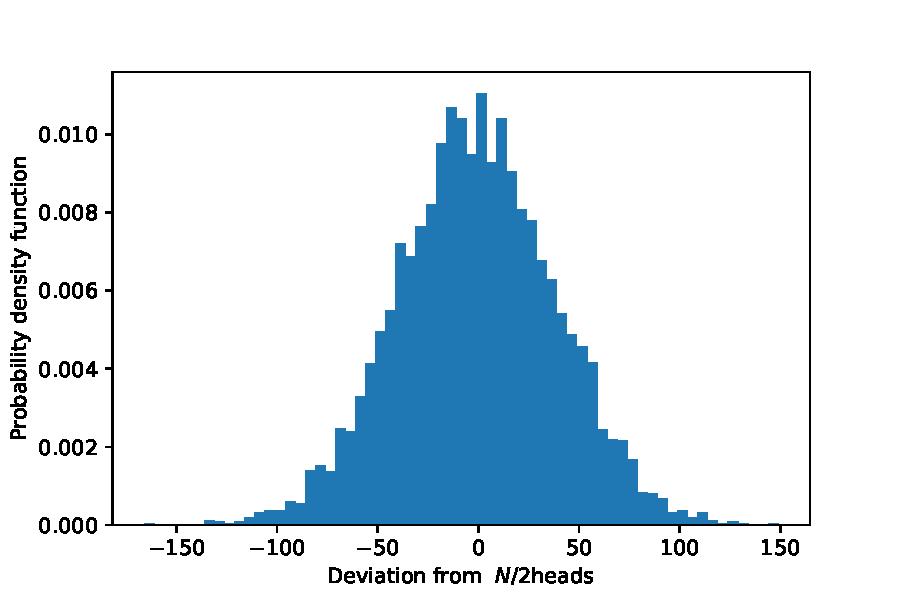
\includegraphics[width=5in]{hist.pdf}
\caption{The histogram}
\end{centering}
\end{figure}

\begin{figure}[H]
\begin{centering}
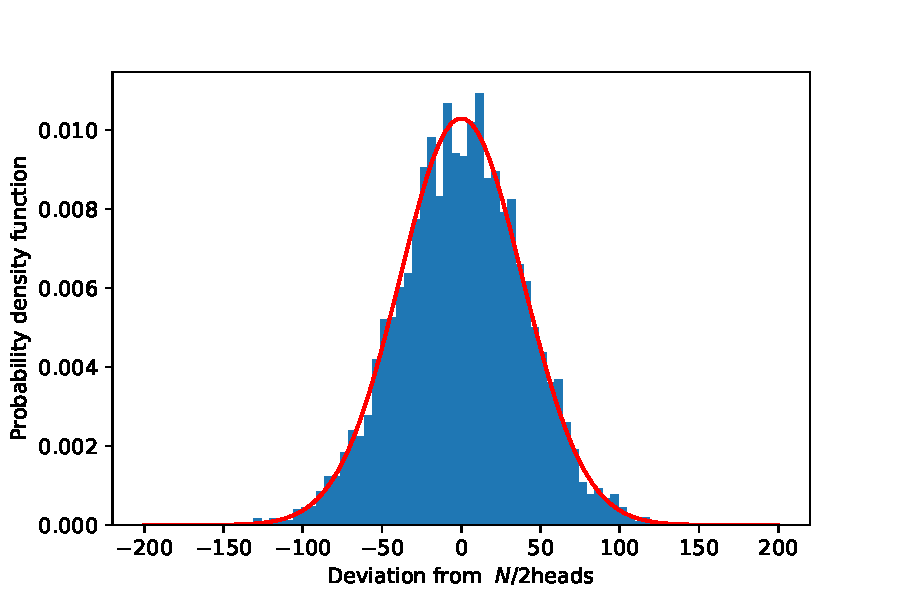
\includegraphics[width=5in]{hist_pdf.pdf}
\caption{The histogram with the probability density function}
\end{centering}
\end{figure}

\item Done in part(a).
\item Done in part(a).
\item It would be a probability distribution which would be accurate near $\frac{N}{2}$.
\item Looking at the Normalization description from the Matlab help page, I think dividing the histogram by the bin width would give us the probability density function.
\item
This code allows us to obtain the width of distribution analytically.


\begin{lstlisting}[style=myPythonstyle]
# September 2017 -- Coin toss
import numpy as np
import matplotlib.pyplot as plt
N_trials = 5000;
Sample_sizes = [2000,3000,6000];
# Note that you can run just one or several Sample_sizes.
# For example, replace the line above with Sample_sizes = [1000, 2000]
# to just have the two Sample_sizes: 1000 and 2000.
width_experimental =[]
width_analytical =[]
for k in Sample_sizes:
	N_samples = k
	Total_heads = []
	for i in range(N_trials):
			# Generate [1 x N_samples] vector of uniformly distributed random
			# integers from 0 or 1.
			rs = np.random.randint(2,size =N_samples);
			# Calculate the total number of heads.
			Total_heads.append(sum(rs));

	BW = 5; # Bin width
	data = np.array(Total_heads)-N_samples/2
	histdata = plt.hist(data,normed=True, bins=np.arange(min(data), max(data) + int(BW), int(BW)))
	x = np.linspace(-200, 200,100) # returns a row vector of 100 evenly spaced points between -200 and 200
	POmega = (1/np.sqrt(np.pi*N_samples/2))*np.exp(-2*(x**2)/N_samples+ -2*(x**2)/N_samples**2);
	plt.plot (x, POmega, 'r-')# 'LineWidth', 2);

	plt.xlabel('Deviation from '+' $N/2$'+'heads');
	plt.ylabel('Probability density function') # Label probability density function


	plt.xlim([-200, 200])



	'''Finding the width'''
	Max_value = max(histdata[0])
	delta =Max_value/20

	elements = np.where(  np.abs(histdata[0]-Max_value/np.exp(1)) <delta)[0]

	width_experimental.append(max(elements[1:]-elements[:-1])*BW) # This is the list of the widths found experimentally
	width_analytical.append(2*N_samples/np.sqrt(2*N_samples+2))

plt.clf()
plt.plot(width_analytical,width_experimental,'r*')
plt.xlabel('Analytical width');
plt.ylabel('Experimental Width')
for xy in zip(width_analytical, width_experimental):                                       # <--
		plt.annotate('(%s, %s)' % xy, xy=xy, textcoords='data') # <--


plt.savefig('widths.pdf')
plt.show()

\end{lstlisting}

The end result is the following plot
\begin{figure}[H]
\begin{centering}
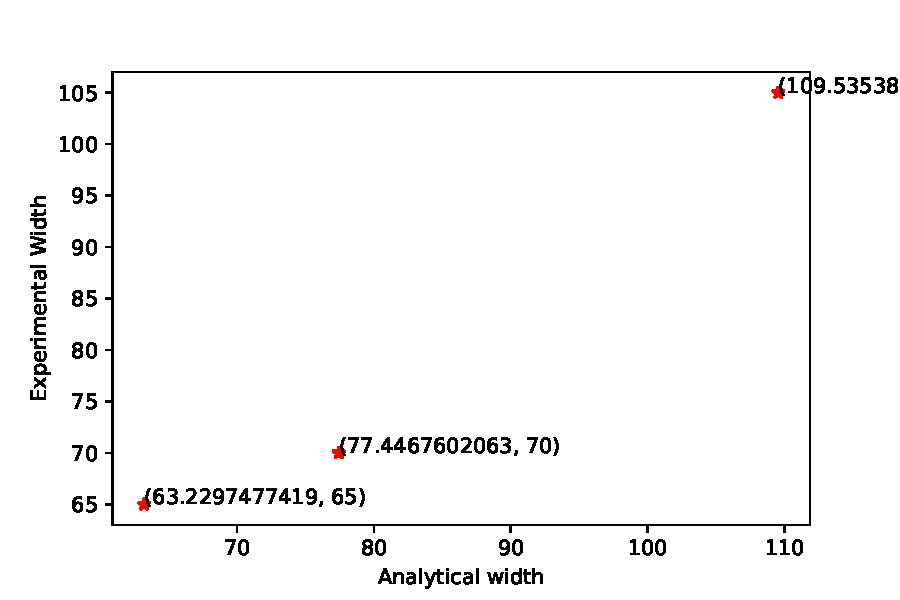
\includegraphics[width=5in]{widths.pdf}
\caption{The widths for 3 distributions}
\end{centering}
\end{figure}

\end{enumerate}

\end{enumerate}
\end{document}
